\chapter{Datos y Preprocesamiento}

Este capítulo describe el análisis y procesamiento de los datos clínicos y administrativos proporcionados por el \textbf{Instituto Nacional de Enfermedades Respiratorias (INER)}. Estos conjuntos de datos están constituidos por registros de admisiones hospitalarias, diagnósticos, comorbilidades y estudios socioeconómicos, los cuales presentan desafíos reales de heterogeneidad, datos faltantes y errores de captura manual.

El uso de estos datos se realizó bajo protocolos de confidencialidad. Se restringió el acceso a información sensible, garantizando que los análisis se centraran en patrones y relaciones detectables sin comprometer la identidad de los pacientes.

\section{Análisis exploratorio y descripción de las bases de datos}

Los datos utilizados en este trabajo de investigación corresponden a registros tabulares de pacientes atendidos durante la emergencia sanitaria por COVID-19, especificamente entre marzo de 2020 y mayo de 2023. La información fue capturada de forma independiente por tres sistemas o departamentos hospitalarios, cada uno con un propósito distinto y sin un mecanismo de integración entre ellos. Esta fragmentación produjo tres bases de datos paralelas que cubren el mismo universo de pacientes, pero que difieren en estructura, volumen y convenciones de captura.

La tabla~\ref{tab:resumen_fuentes} presenta las cifras principales de cada fuente.

\begin{table}[H]
\centering
\caption{Volumen, estructura y propósito por fuente de datos}
\label{tab:resumen_fuentes}
\small
\resizebox{\linewidth}{!}{%
\begin{tabular}{>{\raggedright\arraybackslash}p{2.8cm}
                >{\centering\arraybackslash}p{1.6cm}
                >{\centering\arraybackslash}p{1.6cm}
                >{\raggedright\arraybackslash}p{3.5cm}
                >{\raggedright\arraybackslash}p{5cm}}
\toprule
\textbf{Base} & \textbf{Registros} & \textbf{Columnas} & \textbf{Cobertura temporal} & \textbf{Propósito} \\
\midrule
Diagnóstico y Comorbilidad
  & 4{,}278 & 24
  & Feb 2020 -- Dic 2023
  & Diagnósticos clínicos (texto libre + CIE-10) y comorbilidades \\
\addlinespace
Económico
  & 4{,}632 & 24
  & Ene 2020 -- May 2023
  & Costo de atención hospitalaria, perfil socioeconómico y geográfico \\
\addlinespace
Trabajo Social
  & 14{,}796 & 20
  & Nov 2019 -- May 2023
  & Evaluación social y datos demográficos completos \\
\midrule
\textbf{Total} & \textbf{23{,}706} & & & \\
\bottomrule
\end{tabular}}
\end{table}

\subsection{Diagnóstico y Comorbilidad}

Esta base registra la información clínica del paciente: diagnósticos principal y secundarios, tanto en texto libre como codificados bajo el estándar CIE-10, junto con comorbilidades específicas y agrupaciones clínicas. Sus 24 columnas se agrupan en cuatro categorías: identificadores y fechas del episodio; diagnósticos en texto libre con sus correspondientes códigos CIE-10; comorbilidades agrupadas; y variables binarias que indican la presencia de condiciones específicas como obesidad, diabetes o cardiopatía.

La tabla~\ref{tab:panorama_comorbilidad_tesis} presenta el panorama general de sus columnas.

\begin{table}[H]
\centering
\small
\caption{Panorama general de columnas — Diagnóstico y Comorbilidad}
\label{tab:panorama_comorbilidad_tesis}
\begin{tabular}{lp{3cm}rr}
\toprule
\textbf{Columna} & \textbf{Tipo de dato} & \textbf{\% Nulos} & \textbf{Únicos} \\
\midrule
expediente            & int64   & 0.00\% & 4097 \\
nombre                & str     & 0.00\% & 4150 \\
fechaing              & str     & 0.00\% & 988  \\
fechaegr              & str     & 0.00\% & 982  \\
diagnosticoprincipal  & str     & 0.00\% & 214  \\
cie101                & str     & 0.00\% & 3    \\
diagnostico2          & str     & 31.58\% & 204 \\
cie102                & str     & 31.86\% & 114 \\
diagnostico3          & str     & 63.46\% & 83   \\
cie103                & str     & 63.51\% & 59   \\
diagnostico4          & str     & 89.22\% & 24   \\
cie104                & str     & 89.22\% & 14   \\
dx2                   & str     & 31.86\% & 114 \\
dx3                   & str     & 63.51\% & 59   \\
dx4                   & str     & 89.22\% & 14   \\
obesidad              & float64 & 0.00\% & 2    \\
obesidad1             & float64 & 0.00\% & 2    \\
cardiopatia           & float64 & 0.00\% & 2    \\
comorbi               & str     & 0.00\% & 10   \\
diabetes              & float64 & 0.00\% & 2    \\
nefropatia            & float64 & 0.00\% & 2    \\
eaperge               & float64 & 0.00\% & 2    \\
tephap                & float64 & 0.00\% & 2    \\
comorbicv             & str     & 0.00\% & 5    \\
\bottomrule
\end{tabular}
\end{table}


\subsection{Económico}

Esta base captura los costos de atención hospitalaria, las variables financieras y el perfil socioeconómico y geográfico del paciente. Sus 24 columnas se agrupan en identificadores y fechas del episodio; variables numéricas de estancia, gastos, ingresos y egresos; variables categóricas demográficas (sexo, escolaridad, ocupación); y variables de clasificación socioeconómica y de residencia.

La tabla~\ref{tab:panorama_econo_tesis} presenta el panorama general de sus columnas.

\begin{table}[H]
\centering
\small
\caption{Panorama general de columnas — Económico}
\label{tab:panorama_econo_tesis}
\resizebox{\linewidth}{!}{%
\begin{tabular}{>{\raggedright\arraybackslash}p{8.5cm}>{\raggedright\arraybackslash}p{2.5cm}rr}
\toprule
\textbf{Columna} & \textbf{Tipo de dato} & \textbf{\% Nulos} & \textbf{Únicos} \\
\midrule
EXP                               & str     & 1.73\%  & 4331 \\
NOMBRE\_DEL\_PACIENTE             & str     & 0.00\%  & 4409 \\
SEXO                              & str     & 0.00\%  & 2    \\
EDAD                              & float64 & 0.15\%  & 104  \\
GRUPO\_EDAD                       & str     & 0.15\%  & 18   \\
RESULTADO                         & str     & 26.40\% & 10   \\
ETIQUETAS\_COVID                  & str     & 66.54\% & 42   \\
MOTIVO\_DE\_EGRESO                & str     & 0.39\%  & 4    \\
FECHA\_INGRESO\_INER              & str     & 0.00\%  & 990  \\
FECHA\_DE\_ALTA\_MEJORIA          & str     & 0.00\%  & 953  \\
DIAS\_ESTANCIA                    & int64   & 0.00\%  & 115  \\
GASTO\_TOTAL                      & float64 & 0.00\%  & 4567 \\
GASTO\_DIARIO                     & float64 & 0.00\%  & 4567 \\
TOTAL\_DE\_INGRESOS               & float64 & 15.72\% & 488  \\
TOTAL\_DE\_EGRESOS                & float64 & 20.27\% & 1683 \\
ESCOLARIDAD                       & str     & 24.59\% & 8    \\
OCUPACION                         & str     & 64.81\% & 9    \\
DERECHOHABIENTE\_Y/O\_BENEFICIARIO & str    & 0.00\%  & 20   \\
VULNERABILIDAD\_SOCIOECONOMICA    & bool    & 0.00\%  & 2    \\
NIVEL\_SOCIOECONOMICO             & str     & 13.10\% & 14   \\
ESTADO\_RESIDENCIA                & str     & 0.97\%  & 32   \\
CLAVE\_GEOESTADISTICA\_ESTATAL    & float64 & 1.21\%  & 27   \\
MUNICIPIO\_RESIDENCIA             & str     & 0.97\%  & 293  \\
CLAVE\_GEOESTADISTICA\_MUNICIPAL  & float64 & 1.21\%  & 141  \\
\bottomrule
\end{tabular}}
\end{table}


\subsection{Trabajo Social}

Esta base concentra la evaluación del área de trabajo social junto con datos demográficos completos. Es la más voluminosa de las tres y, a diferencia de las otras, descompone el nombre del paciente en tres campos separados (apellido paterno, apellido materno y nombre de pila). Sus 20 columnas incluyen identificadores del paciente; variables numéricas y categóricas demográficas; y campos de clasificación socioeconómica. Incluye además la columna \texttt{Unnamed: 19}, un artefacto del proceso de extracción con 98.3\% de valores nulos que no aporta información alguna y cuya eliminación es directa, dando paso al análisis de calidad de los datos.

La tabla~\ref{tab:panorama_ts_tesis} presenta el panorama general de las columnas de esta base.

\begin{table}[H]
\centering
\footnotesize
\caption{Panorama general de columnas — Trabajo Social}
\label{tab:panorama_ts_tesis}
\resizebox{\linewidth}{!}{%
\begin{tabular}{>{\raggedright\arraybackslash}p{5.5cm} >{\raggedright\arraybackslash}p{2.5cm} r r}
\toprule
\textbf{Columna} & \textbf{Tipo de dato} & \textbf{\% Nulos} & \textbf{Únicos} \\
\midrule
AÑO                                  & int64   &  0.00\% &      4 \\
FILA                                 & int64   &  0.00\% &  6{,}108 \\
EXPEDIENTE                           & int64   &  0.00\% & 14{,}795 \\
NO. HISTORIA                         & str     &  0.00\% & 14{,}794 \\
FECHA DE ELABORACIÓN                 & str     & 27.85\% &  2{,}333 \\
APELLIDO PATERNO                     & str     &  0.01\% &  3{,}368 \\
APELLIDO MATERNO                     & str     &  0.67\% &  2{,}483 \\
NOMBRE                               & str     &  0.13\% &  6{,}377 \\
EDAD                                 & str     &  4.40\% &  5{,}503 \\
FECHA DE NACIMIENTO                  & str     &  4.40\% & 10{,}999 \\
GENERO                               & str     &  4.51\% &      2 \\
DIAGNOSTICO                          & str     & 61.30\% &    165 \\
ESCOLARIDAD                          & str     &  0.13\% &     49 \\
OCUPACIÓN                            & str     &  4.43\% &    265 \\
DERECHOHABIENTE Y/O BENEFICIARIO     & str     &  1.68\% &     29 \\
DELEGACIÓN O MUNICIPIO PERMANENTE    & str     &  1.70\% &  1{,}073 \\
ESTADO / PAIS PERMANENTE             & str     &  0.05\% &    143 \\
TOTAL DE PUNTOS                      & str     &  0.03\% &     99 \\
NIVEL SOCIOECONÓMICO                 & str     &  0.03\% &     60 \\
\texttt{Unnamed: 19}                 & str     & 98.26\% &      7 \\
\bottomrule
\end{tabular}}
\end{table}


\subsection{Taxonomía de variables por fuente}

La tabla~\ref{tab:taxonomia_funcional} clasifica las columnas de cada fuente combinando tres criterios: el rol que cumple la columna en el registro (identificador, fecha, índice), el tipo de dato que almacena (numérico, binario, texto libre) y el tipo de variable estadística (categórica nominal, continua). Ningún criterio resulta suficiente por sí mismo para agrupar las columnas, pero la combinación de los tres revela patrones estructurales y funcionales de cada sistema de captura.

\begin{table}[H]
\centering
\caption{Clasificación funcional de columnas por fuente}
\label{tab:taxonomia_funcional}
\small
\resizebox{\linewidth}{!}{%
\begin{tabular}{>{\raggedright\arraybackslash}p{3.5cm}
                >{\raggedright\arraybackslash}p{5.5cm}
                >{\raggedright\arraybackslash}p{5.5cm}
                >{\raggedright\arraybackslash}p{5.5cm}}
\toprule
\textbf{Categoría} & \textbf{Comorbilidad} & \textbf{Económico} & \textbf{Trabajo Social} \\
\midrule
Identificadores
  & \texttt{expediente}, \texttt{nombre}
  & \texttt{EXP}, \texttt{NOMBRE\_DEL\_PACIENTE}
  & \texttt{EXPEDIENTE}, \texttt{NO. HISTORIA}, \texttt{APELLIDO PATERNO}, \texttt{APELLIDO MATERNO}, \texttt{NOMBRE} \\
\midrule
Fechas (datetime)
  & \texttt{fechaing}, \texttt{fechaegr}
  & \texttt{FECHA\_INGRESO\_INER}, \texttt{FECHA\_DE\_ALTA\_MEJORIA}
  & \texttt{FECHA DE ELABORACIÓN}, \texttt{FECHA DE NACIMIENTO} \\
\midrule
Numéricos (entero y flotante)
  & ---
  & \texttt{EDAD}, \texttt{DIAS\_ESTANCIA}, \texttt{GASTO\_TOTAL}, \texttt{GASTO\_DIARIO}, \texttt{TOTAL\_DE\_INGRESOS}, \texttt{TOTAL\_DE\_EGRESOS}, \texttt{CLAVE GEOESTADISTICA} (estatal y municipal)
  & \texttt{AÑO}, \texttt{FILA}, \texttt{EDAD}, \texttt{TOTAL DE PUNTOS} \\
\midrule
Binarios (0/1)
  & \texttt{obesidad}, \texttt{obesidad1}, \texttt{cardiopatia}, \texttt{diabetes}, \texttt{nefropatia}, \texttt{eaperge}, \texttt{tephap}
  & \texttt{VULNERABILIDAD\_SOCIOECONOMICA}
  & --- \\
\midrule
Categóricos (baja cardinalidad)
  & \texttt{comorbi}, \texttt{comorbicv}, \texttt{cie101}
  & \texttt{SEXO}, \texttt{RESULTADO}, \texttt{MOTIVO\_DE\_EGRESO}, \texttt{ESCOLARIDAD}, \texttt{OCUPACION}
  & \texttt{GENERO}, \texttt{DERECHOHABIENTE Y/O BENEFICIARIO}, \texttt{ESCOLARIDAD}, \texttt{NIVEL SOCIOECONÓMICO}, \texttt{Unnamed: 19} \\
\midrule
Categóricos (alta cardinalidad)
  & \texttt{cie102--104}, \texttt{dx2--dx4}
  & \texttt{GRUPO\_EDAD}, \texttt{DERECHOHABIENTE Y/O BENEFICIARIO}, \texttt{NIVEL\_SOCIOECONOMICO}, \texttt{ETIQUETAS\_COVID}, \texttt{ESTADO\_RESIDENCIA}, \texttt{MUNICIPIO\_RESIDENCIA}
  & \texttt{OCUPACIÓN}, \texttt{DELEGACIÓN O MUNICIPIO PERMANENTE}, \texttt{ESTADO / PAIS PERMANENTE} \\
\midrule
Texto libre
  & \texttt{diagnosticoprincipal}, \texttt{diagnostico2--4}
  & ---
  & \texttt{DIAGNOSTICO} \\
\bottomrule
\end{tabular}}
\end{table}

La clasificación funcional, aunque útil técnicamente, no refleja el tipo de \emph{información} que las columnas representan. La tabla~\ref{tab:taxonomia_semantica} reagrupa las mismas columnas según su naturaleza semántica, que es la perspectiva relevante para un sistema de ligado de registros: lo que importa es qué columnas son comparables entre fuentes, no cómo están almacenadas.

\begin{table}[H]
\centering
\caption{Clasificación por naturaleza semántica de la información}
\label{tab:taxonomia_semantica}
\small
\resizebox{\linewidth}{!}{%
\begin{tabular}{>{\raggedright\arraybackslash}p{3cm}
                >{\raggedright\arraybackslash}p{5.5cm}
                >{\raggedright\arraybackslash}p{5.5cm}
                >{\raggedright\arraybackslash}p{5.5cm}}
\toprule
\textbf{Naturaleza} & \textbf{Comorbilidad} & \textbf{Económico} & \textbf{Trabajo Social} \\
\midrule
Identificación
  & \texttt{nombre}
  & \texttt{NOMBRE\_DEL\_PACIENTE}, \texttt{SEXO}, \texttt{EDAD}, \texttt{GRUPO\_EDAD}
  & \texttt{APELLIDO PATERNO}, \texttt{APELLIDO MATERNO}, \texttt{NOMBRE}, \texttt{EDAD}, \texttt{FECHA DE NACIMIENTO}, \texttt{GENERO} \\
\midrule
Clínica
  & \texttt{diagnosticoprincipal}, \texttt{diagnostico2--4}, \texttt{cie101--104}, \texttt{dx2--dx4}, \texttt{comorbi}, \texttt{comorbicv}, \texttt{obesidad}, \texttt{obesidad1}, \texttt{cardiopatia}, \texttt{diabetes}, \texttt{nefropatia}, \texttt{eaperge}, \texttt{tephap}
  & \texttt{RESULTADO}, \texttt{ETIQUETAS\_COVID}, \texttt{MOTIVO\_DE\_EGRESO}
  & \texttt{DIAGNOSTICO} \\
\midrule
Geográfica
  & ---
  & \texttt{ESTADO\_RESIDENCIA}, \texttt{MUNICIPIO\_RESIDENCIA}, \texttt{CLAVE GEOESTADISTICA} (estatal y municipal)
  & \texttt{DELEGACIÓN O MUNICIPIO PERMANENTE}, \texttt{ESTADO / PAIS PERMANENTE} \\
\midrule
Socioeconómica
  & ---
  & \texttt{ESCOLARIDAD}, \texttt{OCUPACION}, \texttt{DERECHOHABIENTE Y/O BENEFICIARIO}, \texttt{NIVEL\_SOCIOECONOMICO}, \texttt{VULNERABILIDAD\_SOCIOECONOMICA}
  & \texttt{ESCOLARIDAD}, \texttt{OCUPACIÓN}, \texttt{DERECHOHABIENTE Y/O BENEFICIARIO}, \texttt{TOTAL DE PUNTOS}, \texttt{NIVEL SOCIOECONÓMICO} \\
\midrule
Administrativa
  & \texttt{expediente}, \texttt{fechaing}, \texttt{fechaegr}
  & \texttt{EXP}, \texttt{DIAS\_ESTANCIA}, \texttt{FECHA\_INGRESO\_INER}, \texttt{FECHA\_DE\_ALTA\_MEJORIA}, \texttt{TOTAL\_DE\_INGRESOS}, \texttt{TOTAL\_DE\_EGRESOS}, \texttt{GASTO\_TOTAL}, \texttt{GASTO\_DIARIO}
  & \texttt{EXPEDIENTE}, \texttt{NO. HISTORIA}, \texttt{FECHA DE ELABORACIÓN}, \texttt{AÑO}, \texttt{FILA} \\
\bottomrule
\end{tabular}}
\end{table}

De esta taxonomía se desprenden cuatro observaciones estructurales clave:

\begin{itemize}
    \item \textbf{Comorbilidad} concentra la información clínica más rica: variables binarias de comorbilidad y doble representación de diagnósticos (texto libre y códigos CIE-10). Es la única fuente con cobertura completa en todas sus columnas clínicas.

    \item \textbf{Económico} es la única fuente con variables financieras cuantitativas y cobertura geográfica codificada (estado, municipio, claves geoestadísticas). Sus campos de diagnóstico son categóricos de baja a media cardinalidad, no texto libre.

    \item \textbf{Trabajo Social} es la única que descompone el nombre en tres campos separados, y la única con índices administrativos (\texttt{AÑO}, \texttt{FILA}) que son artefactos de consolidación temporal, sin valor semántico.

    \item \textbf{El orden del nombre difiere entre Comorbilidad y Económico.} Comorbilidad almacena \texttt{NOMBRE(S) APELLIDO\_P APELLIDO\_M}, mientras que Económico lo invierte a \texttt{APELLIDO\_P APELLIDO\_M NOMBRE(S)}. Trabajo Social evita esta ambigüedad separando los tres componentes en campos distintos.
\end{itemize}

La tabla~\ref{tab:cardinalidad_compartidos} profundiza en los campos categóricos que aparecen tanto en Económico como en Trabajo Social, mostrando cómo la cardinalidad se reduce ---o no--- al normalizar el texto.

\begin{table}[H]
\centering
\caption{Cardinalidad de campos compartidos --- Económico vs.\ Trabajo Social}
\label{tab:cardinalidad_compartidos}
\small
\resizebox{\linewidth}{!}{%
\begin{tabular}{>{\raggedright\arraybackslash}p{6.0cm}
                >{\centering\arraybackslash}p{2.2cm}
                >{\centering\arraybackslash}p{2.2cm}
                >{\centering\arraybackslash}p{2.2cm}
                >{\centering\arraybackslash}p{2.2cm}
                >{\raggedright\arraybackslash}p{2.2cm}}
\toprule
\textbf{Campo} & \textbf{Cat.\ Econo.} & \textbf{Cat.\ norm.\ Econo.} & \textbf{Cat.\ TS} & \textbf{Cat.\ norm.\ TS} \\
\midrule
ESCOLARIDAD                      &  8 &  6 &  49 & 25  \\
OCUPACIÓN                        &  9 &  8 & 265 & 265 \\
DERECHOHABIENTE Y/O BENEFICIARIO & 20 & 20 &  29 &  23 \\
NIVEL SOCIOECONÓMICO             & 14 & 14 &  60 &  60 \\
\bottomrule
\end{tabular}}
\end{table}

El contraste más extremo es \texttt{OCUPACIÓN}: Económico emplea un vocabulario controlado con 9 categorías, mientras que Trabajo Social lo captura como texto libre de alta cardinalidad que no se reduce tras normalización. \texttt{DERECHOHABIENTE Y/O BENEFICIARIO} concentra la mayoría de sus registros en variantes del mismo valor (\texttt{Ninguno}, \texttt{NINGUNO}, \texttt{Ninguno} con espacio final), generando cardinalidad artificial sin diferencia semántica. \texttt{NIVEL SOCIOECONÓMICO} usa escalas incompatibles entre fuentes: sufijos \texttt{E}/\texttt{X} en Económico frente a una escala numérica propia en Trabajo Social.

\subsection{Cobertura de valores nulos}
Algo sumamente relevante para el proceso de ligado es la completitud de la información presente en cada registro. En particular, las bases de datos analizadas presentan una alta ausencia de datos que varían entre campo sin patrones claros.

La tabla~\ref{tab:nulos_comparativo} resume los patrones de nulos más relevantes por categoría de campo y fuente.

\begin{table}[H]
\centering
\caption{Patrones de valores nulos por campo y base de datos}
\label{tab:nulos_comparativo}
\small
\resizebox{\linewidth}{!}{%
\begin{tabular}{>{\raggedright\arraybackslash}p{6cm}
                >{\centering\arraybackslash}p{3cm}
                >{\centering\arraybackslash}p{3.5cm}
                >{\centering\arraybackslash}p{3.5cm}}
\toprule
\textbf{Campo / Categoría} & \textbf{Comorbilidad} & \textbf{Económico} & \textbf{Trabajo Social} \\
\midrule
Expediente & 0\% & 1.73\% (80 regs.) & 0\% \\
\midrule
Nombre (identificación) & 0\% & 0\% & $<$1\% \\
\midrule
Fecha de ingreso/elaboración & 0\% & 0\% & 27.85\% \\
\midrule
Fecha de egreso/alta & 0\% & 0\% & --- \\
\midrule
Diagnóstico principal & 0\% & 26.4\% & 61.3\% \\
\midrule
Diagnósticos adicionales & 31.6\%--89.2\% & --- & --- \\
\midrule
Clasificación COVID & --- & 66.5\% & --- \\
\midrule
Variables socioeconómicas & --- & 13.1\%--64.8\% & $<$5\% \\
\midrule
Variables geográficas & --- & $<$2\% & $<$2\% \\
\midrule
Variables demográficas & --- & $<$1\% & 4.4\%--4.5\% \\
\bottomrule
\end{tabular}}
\end{table}

Se distinguen tres patrones de ausencia de datos:

\textbf{Patrón 1---Nulos estructurales:} En Comorbilidad, los diagnósticos secundario, terciario y cuarto son nulos cuando el paciente no registró diagnósticos adicionales, por lo que su ausencia es informativa. En Trabajo Social, \texttt{DIAGNOSTICO} solo tiene valor en registros del periodo COVID-19, y \texttt{Unnamed: 19} es un artefacto del sistema con cobertura casi nula, candidato directo a eliminación.

\textbf{Patrón 2---Nulos por cobertura parcial:} En Económico, los nulos de \texttt{ETIQUETAS\_COVID} se concentran en registros más antiguos (incorporación tardía del campo), mientras que los de \texttt{RESULTADO} aparecen distribuidos uniformemente (captura inconsistente). \texttt{EXP} es el único identificador primario con valores faltantes en todo el conjunto de datos.

\textbf{Patrón 3---Nulos por falta de captura:} \texttt{FECHA DE ELABORACIÓN} en Trabajo Social, y \texttt{ESCOLARIDAD} y \texttt{OCUPACION} en Económico presentan alta ausencia de datos por inconsistencia en el proceso de registro, no por diseño del sistema.


En conjunto suman 23,706 registros distribuidos en tres esquemas que comparten información del mismo paciente pero desde perspectivas distintas. Ninguna base cuenta con un identificador único universal: el número de expediente es el campo candidato a llave, pero su nomenclatura y confiabilidad varían entre fuentes. Los campos de nombre del paciente presentan diferencias de orden (el formato \texttt{NOMBRE APELLIDOS} en Comorbilidad frente a \texttt{APELLIDOS NOMBRE} en Económico), de estructura (campos separados en Trabajo Social frente a campo único en las otras dos) y de codificación de caracteres. Esta heterogeneidad estructural es el eje del problema que este trabajo aborda: ante la ausencia de un identificador común confiable, se requiere un mecanismo de comparación que opere directamente sobre la información disponible, trascendiendo las variaciones superficiales de captura entre los tres sistemas.

\section{Calidad de los datos y heterogeneidad estructural}

El análisis de calidad se organiza alrededor de los campos que afectan directamente la identificación del paciente y el proceso de ligado entre fuentes. Se examinan primero los campos críticos comparables entre las tres bases ---\textbf{nombre}, \textbf{expediente} y \textbf{fechas}--- y se consolidan al final los hallazgos específicos de cada fuente.

\subsection{Campo nombre}

El campo de nombre del paciente es el más heterogéneo en calidad entre las tres fuentes. A las diferencias de formato ya documentadas se suman patrones de degradación distintos en cada sistema. La tabla~\ref{tab:chars_nombre} resume los caracteres problemáticos detectados en los campos de nombre de cada base.

\begin{table}[H]
\centering
\caption{Caracteres problemáticos en campos de nombre por fuente}
\label{tab:chars_nombre}
\small
\resizebox{\linewidth}{!}{%
\begin{tabular}{>{\raggedright\arraybackslash}p{2.5cm}
                >{\raggedright\arraybackslash}p{4.0cm}
                >{\centering\arraybackslash}p{2.2cm}
                >{\centering\arraybackslash}p{2.5cm}
                >{\raggedright\arraybackslash}p{5.0cm}}
\toprule
\textbf{Fuente} & \textbf{Campo(s)} & \textbf{Registros} & \textbf{\%} & \textbf{Caracteres principales} \\
\midrule
Comorbilidad
  & \texttt{nombre}
  & 307
  & 7.2\%
  & \texttt{?} por Ñ (223), punto (85), \texttt{|} (3) \\
\addlinespace
Económico
  & \texttt{NOMBRE\_DEL\_PACIENTE}
  & 78
  & 1.7\%
  & punto (49), paréntesis con anotación clínica (28), \texttt{/} (1) \\
\addlinespace
Trabajo Social
  & \texttt{AP. PATERNO} / \texttt{AP. MATERNO} / \texttt{NOMBRE}
  & 99 / 39 / 181
  & 0.7\% / 0.3\% / 1.2\%
  & punto (225), NBSP (58), \texttt{/} (32), \texttt{|} (3) \\
\bottomrule
\end{tabular}}
\end{table}

Cada fuente presenta un tipo de problema distinto. En \textbf{Comorbilidad}, la causa dominante es un error de encoding del sistema fuente: el carácter \texttt{?} representa una Ñ mal codificada (ej. \texttt{RAMIREZ NI?O} por \texttt{RAMIREZ NIÑO}), corregible mediante una regla simple de sustitución. En \textbf{Económico}, el problema principal es la captura de anotaciones clínicas dentro del campo de nombre (\texttt{CAMACHO ROJAS MARIA (ESAVI)}), que requiere limpieza mediante expresión regular. En \textbf{Trabajo Social}, el carácter más problemático es el espacio de no separación NBSP (\textbackslash xa0), que no es detectado por la función estándar \texttt{strip()}; el punto abreviativo (\texttt{MA. CARMEN}) y el prefijo \texttt{R/N} son convenciones de captura más que errores.

\subsection{Campo expediente}

El número de expediente es el principal candidato a llave foránea para el ligado entre fuentes. La tabla~\ref{tab:exp_calidad} resume las métricas clave de cada fuente.

\begin{table}[H]
\centering
\caption{Calidad del identificador de expediente por fuente}
\label{tab:exp_calidad}
\small
\resizebox{\linewidth}{!}{%
\begin{tabular}{>{\raggedright\arraybackslash}p{2.5cm}
                >{\raggedright\arraybackslash}p{1.8cm}
                >{\centering\arraybackslash}p{2cm}
                >{\centering\arraybackslash}p{1.5cm}
                >{\centering\arraybackslash}p{2.2cm}
                >{\centering\arraybackslash}p{2.5cm}
                >{\raggedright\arraybackslash}p{3.0cm}}
\toprule
\textbf{Fuente} & \textbf{Campo} & \textbf{Cobertura} & \textbf{Únicos} & \textbf{EXP dup.} & \textbf{Conflictos EXP$\leftrightarrow$nombre} & \textbf{Rango} \\
\midrule
Comorbilidad & \texttt{expediente} & 100\% & 95.8\% & 159 (340 regs.) & 14 (tipográficos) & 76,389--255,242 \\
\addlinespace
Económico    & \texttt{EXP}        & 98.3\% & 93.5\% & 173 (394 regs.) & 6 (identidades distintas) & 76,389--684,189 \\
\addlinespace
Trabajo Social & \texttt{EXPEDIENTE} & 100\% & 100\% & 1 (2 regs.) & 0 & 236,215--251,119 \\
\bottomrule
\end{tabular}}
\end{table}

Las tres fuentes difieren en su confiabilidad como llave foránea de forma gradual. \textbf{Trabajo Social} es el más limpio: cobertura perfecta, prácticamente sin duplicados, cero conflictos con nombre y un rango numérico compacto que sugiere un subsistema de asignación propio. Cuenta además con un segundo identificador, \texttt{NO. HISTORIA} (formato \texttt{IAN\#\#\#\#\#\#}), utilizable como respaldo.

\textbf{Comorbilidad} presenta expedientes duplicados por reingresos (el mismo paciente atendido más de una vez). Los conflictos entre expediente y nombre son artefactos tipográficos o de codificación del mismo episodio, no identidades distintas. El rango mínimo coincide con el de Económico, lo que indica un sistema de asignación compartido entre ambas fuentes.

\textbf{Económico} es el más problemático: además de duplicados por reingresos, presenta registros con \texttt{EXP} nulo o con valor \texttt{S/E} que no pueden participar en ningún ligado vía este campo, y expedientes asignados a personas con nombres completamente distintos en fechas próximas. Estos casos constituyen errores del sistema de captura, no artefactos de normalización, y hacen que \texttt{EXP} no pueda emplearse como llave única sin validación cruzada con el campo de nombre.

\subsection{Fechas}

Las tres fuentes no comparten la misma estructura de campos de fecha, lo que condiciona el tipo de verificación posible en cada una. La tabla~\ref{tab:fechas_calidad} resume la cobertura y los hallazgos por fuente.

\begin{table}[H]
\centering
\caption{Campos de fecha y hallazgos de coherencia por fuente}
\label{tab:fechas_calidad}
\small
\resizebox{\linewidth}{!}{%
\begin{tabular}{>{\raggedright\arraybackslash}p{2.5cm}
                >{\raggedright\arraybackslash}p{4.0cm}
                >{\centering\arraybackslash}p{2.5cm}
                >{\raggedleft\arraybackslash}p{6cm}}
\toprule
\textbf{Fuente} & \textbf{Campos de fecha} & \textbf{Nulos} & \textbf{Hallazgos} \\
\midrule
Comorbilidad
  & \texttt{fechaing}, \texttt{fechaegr}
  & 0 en ambos
  & 0 fuera de rango; 0 inversiones; 19 ingresos igual a egreso (altas mismo día) \\
\addlinespace
Económico
  & \texttt{FECHA\_INGRESO\_INER}, \texttt{FECHA\_DE\_ALTA\_MEJORIA}
  & 0 en ambos
  & 8 altas anteriores al ingreso (inversión); 143 mismo día; 12 discrepancias con \texttt{DIAS\_ESTANCIA} \\
\addlinespace
Trabajo Social
  & \texttt{FECHA DE ELABORACIÓN}, \texttt{FECHA DE NACIMIENTO}
  & 4,120 / 651
  & 2 registros con fecha 2019 (atípicos); valor mínimo de nacimiento 1916 (posible captura errónea) \\
\bottomrule
\end{tabular}}
\end{table}

\textbf{Comorbilidad} es la fuente con la mayor limpieza temporal: cobertura completa, ningún registro fuera del rango COVID y altas el mismo día del ingreso que son clínicamente posibles.

\textbf{Económico} presenta el único caso de inversión temporal entre las tres fuentes: registros con \texttt{FECHA\_DE\_ALTA\_MEJORIA} anterior a \texttt{FECHA\_INGRESO\_INER}, concentrados en enero--marzo de 2020, lo que sugiere un valor por defecto del sistema al inicio de la pandemia. Algunos de estos registros generan un \texttt{DIAS\_ESTANCIA} negativo, confirmando la anomalía. Las discrepancias adicionales entre días calculados y el campo \texttt{DIAS\_ESTANCIA} son menores (diferencia de un día por criterio de conteo).

\textbf{Trabajo Social} tiene una estructura de fechas cualitativamente distinta: no registra ingreso ni egreso clínico, sino la fecha de elaboración de la valoración social, que es el campo con mayor proporción de nulos entre todas las fechas del conjunto. La fecha de nacimiento tiene un valor mínimo sospechoso que podría indicar errores de captura en pacientes de edad avanzada. El campo \texttt{AÑO} codifica el año de forma redundante y debe descartarse.

\subsection{Anomalías y hallazgos específicos por fuente}

A diferencia de los campos anteriores ---nombre, expediente y fechas, que permiten una comparación directa entre fuentes--- las columnas restantes de cada base no tienen contraparte en las otras dos. Cada fuente captura dimensiones distintas: diagnósticos clínicos codificados (Comorbilidad), variables financieras y socioeconómicas con vocabulario controlado (Económico), y variables socioeconómicas con captura libre más campos administrativos de consolidación (Trabajo Social). Los hallazgos de calidad se presentan por separado para cada una.

\textbf{Comorbilidad.}
\begin{itemize}
    \item \textbf{Códigos fuera del catálogo oficial CIE-10.} \texttt{cie101} (diagnóstico principal) es 100\% conforme al estándar. Los diagnósticos secundario y terciario presentan extensiones institucionales propias del hospital: \texttt{cie102} con 13.4\%, \texttt{cie103} con 28.5\% y \texttt{cie104} con 5.2\% de códigos no catalogados en el estándar ISO. Tienen significado clínico real en el contexto institucional y no deben tratarse como errores, aunque requieren un mapeo explícito antes de cualquier análisis comparativo externo.

    \item \textbf{Redundancia total de columnas \texttt{dx}.} Las columnas \texttt{dx2}, \texttt{dx3} y \texttt{dx4} son duplicados exactos (100\% de coincidencia registro a registro) de \texttt{cie102}, \texttt{cie103} y \texttt{cie104} respectivamente, incluyendo los mismos patrones de nulos. Son candidatas directas a eliminación.

    \item \textbf{Alta variabilidad textual en diagnósticos libres.} \texttt{diagnosticoprincipal} presenta cientos de variantes textuales que se colapsan a apenas tres códigos CIE-10, con \texttt{U07.1} (COVID-19) dominando casi la totalidad de los registros. Esta variabilidad justifica el uso del código CIE-10 como referencia canónica.

    \item \textbf{Discordancia \texttt{obesidad} vs \texttt{obesidad1}.} Ambas columnas registran obesidad pero difieren en el 13.7\% de los registros. En todos los casos discordantes \texttt{obesidad}=1 y \texttt{obesidad1}=0, lo que indica que \texttt{obesidad} aplica un criterio clínico más amplio.

    \item \textbf{Consistencia interna de las variables de agrupación.} Las categorías de \texttt{comorbi} y \texttt{comorbicv} son internamente coherentes con las variables binarias individuales que agrupan.
\end{itemize}

\textbf{Económico.}
\begin{itemize}
    \item \textbf{Valores extremos en variables financieras.} \texttt{GASTO\_TOTAL} y \texttt{GASTO\_DIARIO} presentan valores superiores a \$2,000,000 MXN y \$61,198/día respectivamente. Corresponden a estancias prolongadas o procedimientos de alta complejidad, no a errores de captura, pero deben considerarse en cualquier modelo que incluya estas variables.

    \item \textbf{Formato mixto en \texttt{EDAD}.} Algunos registros presentan edad fuera del rango esperado: bebés menores de un año registrados como fracción decimal (ej. 0.833 = 10 meses) y un valor extremo de 104 años que probablemente es un error de captura.

    \item \textbf{Inconsistencias en variables categóricas.} La normalización reduce categorías en \texttt{ESCOLARIDAD} y \texttt{OCUPACION} únicamente por espacios finales. \texttt{ETIQUETAS\_COVID} refleja su incorporación tardía al sistema de captura. \texttt{MUNICIPIO\_RESIDENCIA} presenta 141 singletons sobre 293 categorías, indicando alta dispersión geográfica.
\end{itemize}

\textbf{Trabajo Social.}
\begin{itemize}
    \item \textbf{\texttt{EDAD} como texto libre.} A diferencia de Económico, la edad se almacena como cadena en formato ``X años Y meses Z días'' (43.4\% con formato completo) o variante parcial (56.6\%). Se detectaron 119 casos extremos: bebés con 0 años expresados en meses y días, y un registro de 102 años que requiere verificación.

    \item \textbf{\texttt{FILA} como artefacto de consolidación.} Este campo es un índice de renglón heredado de los archivos anuales que forman el CSV consolidado. Cada valor aparece entre una y cuatro veces según cuántos archivos contenían ese número de fila, sin ningún significado clínico ni administrativo.

    \item \textbf{\texttt{OCUPACIÓN} como campo de captura libre.} Se comporta como texto libre con alta cardinalidad (61 singletons), en contraste con el vocabulario controlado del campo homónimo en Económico.

    \item \textbf{Alta cardinalidad geográfica.} \texttt{DELEGACIÓN O MUNICIPIO PERMANENTE} pasa de 1,073 a 759 categorías tras normalización, con 514 singletons. La reducción refleja variaciones tipográficas, pero la cardinalidad residual es demasiado alta para tratamiento como variable categórica directa.
\end{itemize}

\section{Generación del conjunto de datos etiquetados}

El espacio de búsqueda \textbf{completo} en el proceso de ligado consta de todos los pares posibles entre registros de las distintas bases de datos. Con un total de 23,706 registros distribuidos en las tres bases, el \textit{producto cartesiano} entre pares de CSV arroja una cifra de \textbf{151,648,056 combinaciones posibles}. Evaluar cada par de forma individual es computacionalmente inviable y de difícil manejo, por lo que se requiere un mecanismo de filtrado que reduzca el espacio a un conjunto manejable de candidatos, algo que la literatura de ligado de registros denomina \emph{blocking} y siempre se realiza como primer paso pues permite descartar de forma relativamente confiable la gran mayoría de los pares que no pueden corresponder a la misma entidad.

El número de expediente, pese a no ser un identificador 100\% confiable, permite un filtro natural: solo se consideran candidatos los pares de registros que comparten el mismo expediente entre dos fuentes distintas, aceptando como limitación no detectar los casos borde donde el expediente no es igual pese a compartir otros atributos, pero permite sugerir patrones estructurales y semánticos que puedan ser útiles para trascender esta limitación hacia nuevas aproximaciones. Este criterio reduce el espacio de 151 millones a 11,424 candidatos. Se añadieron 63 pares adicionales correspondientes a registros de la base Económico cuyo expediente es nulo pero cuyo nombre normalizado coincide con el de otra fuente, totalizando 11,487 pares candidatos.

\subsection{Vinculación inicial}

Como primer paso se aplicó una normalización básica: conversión a mayúsculas, eliminación de acentos y colapso de espacios. Con esta versión se construyeron pares (expediente, nombre) por cada base y se compararon en los tres cruces posibles. La tabla~\ref{tab:vinculacion_basica} muestra los resultados.

\begin{table}[H]
\centering
\caption{Vinculación entre bases --- normalización básica}
\label{tab:vinculacion_basica}
\resizebox{\textwidth}{!}{%
\begin{tabular}{>{\raggedright\arraybackslash}p{3.8cm} >{\centering\arraybackslash}p{1.3cm} >{\centering\arraybackslash}p{1.3cm} >{\centering\arraybackslash}p{1.5cm} >{\centering\arraybackslash}p{1.8cm} >{\centering\arraybackslash}p{2.0cm} >{\centering\arraybackslash}p{2.3cm}}
\toprule
\textbf{Cruce} & \textbf{EXP A} & \textbf{EXP B} & \textbf{EXP iguales} & \textbf{Nombres iguales} & \textbf{EXP y nombre iguales} & \textbf{EXP igual, nombre distinto} \\
\midrule
Económico $\leftrightarrow$ Comorbilidad   & 4{,}330 &  4{,}097 & 3{,}629 &     1 &     1 & 3{,}628 \\
Económico $\leftrightarrow$ Trabajo Social  & 4{,}330 & 14{,}795 & 3{,}995 & 3{,}661 & 3{,}653 &   342 \\
Comorbilidad $\leftrightarrow$ Trabajo Social & 4{,}097 & 14{,}795 & 3{,}800 &    17 &    16 & 3{,}784 \\
\bottomrule
\end{tabular}%
}
\end{table}



El resultado revela un problema severo: el cruce Económico $\leftrightarrow$ Comorbilidad, que comparte 3,629 expedientes, apenas registra un par con nombre coincidente; los 3,628 restantes aparecen con nombres distintos a pesar de compartir expediente. El cruce Comorbilidad $\leftrightarrow$ Trabajo Social presenta un patrón similar, con 3,784 discrepancias de 3,800 expedientes compartidos. En contraste, Económico $\leftrightarrow$ Trabajo Social muestra una alta tasa de coincidencia (3,653 de 3,995), lo que sugiere que el problema no es la calidad de los nombres en sí, sino la forma en que se almacenan entre sistemas.

La tabla~\ref{tab:disc_v1_econ_comor} presenta una muestra de las discrepancias para el cruce más afectado.

\begin{table}[H]
\centering
\small
\caption{Muestra de discrepancias --- Económico $\leftrightarrow$ Comorbilidad}
\label{tab:disc_v1_econ_comor}
\resizebox{\linewidth}{!}{%
\begin{tabular}{r >{\raggedright\arraybackslash}p{8cm} >{\raggedright\arraybackslash}p{8cm}}
\toprule
\textbf{EXP} & \textbf{Nombre (Económico)} & \textbf{Nombre (Comorbilidad)} \\
\midrule
237568 & MOLINA GONZALEZ BLANCA ESTELA     & BLANCA ESTELA MOLINA GONZALEZ \\
237569 & MENDEZ AGUILAR JOSE ODILON MAR    & JOSE ODILON MAR MENDEZ AGUILAR \\
237571 & GARCIA MARTINEZ DONACIANO         & DONACIANO GARCIA MARTINEZ \\
237572 & CALDERON REYES CONSUELO           & CONSUELO CALDERON REYES \\
237574 & PRADO APOLINAR VICTOR DANIEL      & DANIEL PRADO APOLINAR \\
237577 & ROSAS CHAVARRIA GUILLERMO         & GUILLERMO ROSAS CHAVARRIA \\
237578 & VIDAL SEGUNDO ESTEBAN             & ESTEBAN VIDAL SEGUNDO \\
237579 & GARDUNO TREJO ALEJANDRO           & ALEJANDRO GARDU?O TREJO \\
237581 & GUADARRAMA PINA MARIA DEL CARME   & MARIA DEL CARME GUADARRAMA PI?A \\
237582 & CASADO CORONA JUAN JOSE           & JUAN JOSE CASADO CORONA \\
\bottomrule
\end{tabular}}
\end{table}



El patrón es claro: Comorbilidad captura el nombre en orden \texttt{NOMBRE AP AM}, mientras que Económico utiliza \texttt{AP AM NOMBRE}. Los tokens son los mismos, solo cambia su orden. Este hallazgo, junto con la codificación defectuosa \texttt{?} por \texttt{Ñ} en Comorbilidad, explica las tasas artificialmente bajas de la vinculación inicial y motiva el diseño de una normalización más robusta.

\subsection{Normalización robusta}

A partir del diagnóstico anterior se diseñó un proceso de normalización que resuelve los problemas sistemáticos en una sola pasada. La normalización consta de cuatro pasos: (1) corrección del encoding defectuoso \texttt{?}$\to$\texttt{N} en la base Comorbilidad, (2) descomposición NFD para eliminar acentos y diacríticos, (3) eliminación de todo carácter no alfabético mediante expresión regular y (4) ordenamiento alfabético de los tokens resultantes. Este último paso hace que la comparación sea invariante al orden de captura del nombre, resolviendo la diferencia estructural entre los formatos \texttt{NOMBRE AP AM} y \texttt{AP AM NOMBRE} que presentan las fuentes.

La tabla~\ref{tab:normalizacion} muestra el impacto de esta normalización en los pares confirmados por la llave exacta: expediente + nombre normalizado iguales.

\begin{table}[H]
\centering
\small
\caption{Pares confirmados: normalización básica vs.\ robusta}
\label{tab:normalizacion}
\begin{tabular}{lrrr}
\toprule
\textbf{Cruce} & \textbf{Básica} & \textbf{Robusta} & \textbf{\% Reconciliados} \\
\midrule
Económico $\leftrightarrow$ Comorbilidad   &     1 & 2,939 & 81.0\% \\
Económico $\leftrightarrow$ Trabajo Social & 3,653 & 3,729 & 93.3\% \\
Comorbilidad $\leftrightarrow$ Trabajo Social & 16 & 3,187 & 83.9\% \\
\bottomrule
\end{tabular}
\end{table}

\subsection{Clasificación por etapas}

La vinculación oficial clasifica los 11,487 candidatos aplicando tres criterios en secuencia. La tabla~\ref{tab:ground_truth} desglosa el resultado de cada capa por cruce entre bases.

\begin{table}[H]
\centering
\small
\caption{Vinculación oficial: pares confirmados por capa y cruce}
\label{tab:ground_truth}
\resizebox{\linewidth}{!}{%
\begin{tabular}{lrrrrr}
\toprule
\textbf{Cruce} & \textbf{\shortstack{Llave\\ exacta}} & \textbf{\shortstack{Métrica\\ clásica}} & \textbf{\shortstack{Rev. manual:\\ match}} & \textbf{\shortstack{Rev. manual:\\ no\_match}} & \textbf{\shortstack{Positivos\\ confirmados}} \\
\midrule
Económico $\leftrightarrow$ Comorbilidad   & 2,939 &   469 & 228 &  9 & 3,636 \\
Económico $\leftrightarrow$ Trabajo Social  & 3,729 &   234 &  59 & 10 & 4,022 \\
Comorbilidad $\leftrightarrow$ Trabajo Social & 3,187 &   415 & 206 &  2 & 3,808 \\
\midrule
\textbf{Total} & \textbf{9,855} & \textbf{1,118} & \textbf{493} & \textbf{21} & \textbf{11,466} \\
\bottomrule
\end{tabular}}
\end{table}

\begin{enumerate}
    \item \textbf{Llave exacta}: resuelve 9,855 pares (85.8\% de los candidatos) al exigir coincidencia perfecta en expediente y nombre normalizado.
    \item \textbf{Métrica clásica}: añade 1,118 pares mediante similitud de Jaro-Winkler ($\text{JW} \geq 0.88$) y distancia de Levenshtein ($\text{Lev} \geq 0.85$), umbrales calibrados manualmente para tolerar errores tipográficos asociados a registros de la misma entidad.
    \item \textbf{Revisión manual}: procesó los 514 pares no resueltos por ninguna de las capas anteriores: 493 se confirmaron como positivos y 21 como negativos.
\end{enumerate}



Las discrepancias que la segunda y tercera capa debieron resolver se agrupan en tres categorías:
\begin{itemize}
    \item \textbf{Errores tipográficos}: variaciones ortográficas menores (\texttt{BERNANDO} vs \texttt{BERNARDO}, \texttt{STEINNER} vs \texttt{STENNER}).
    \item \textbf{Nombres truncados o incompletos}: una fuente registra el nombre completo y la otra solo una abreviación (\texttt{MAR} vs \texttt{MARIO}, \texttt{CARME} vs \texttt{CARMEN}).
    \item \textbf{Nombres sustancialmente distintos para el mismo expediente}: atribuibles a posibles errores de captura o reasignación de expediente en el sistema hospitalario (e.g., \texttt{VICTOR DANIEL} vs \texttt{ARMANDO} en el EXP 237574).
\end{itemize}
Las dos primeras categorías fueron resueltas mayoritariamente por la capa de métrica clásica; la tercera requirió revisión manual a detalle para determinar si los registros correspondían al mismo paciente.

El resultado es un conjunto de 11,466 pares positivos que constituye un \textbf{estándar de plata} (\textit{silver standard}): es decir, un conjunto de datos etiquetado mediante reglas deterministas, no por revisión exhaustiva, suficiente para entrenar y evaluar los modelos de aprendizaje profundo de los capítulos subsecuentes aunque con posible ruido inherente a la vinculación automática. Los 21 pares negativos confirmados se conservan como referencia de alta calidad, aunque su volumen es marginal frente al desbalance natural del problema.

\subsection{Resolución de entidades}

El concepto central de la vinculación es la \textbf{entidad}: la representación unificada de un paciente real a través de sus distintas apariciones en las bases de datos. Cada entidad agrupa uno o más registros confirmados como pertenecientes al mismo paciente y recibe un identificador numérico único: \texttt{entity\_id}.

La Tabla~\ref{tab:ejemplo_entidades} ilustra el concepto: dos registros con nombres ligeramente distintos por error de captura quedan agrupados bajo el mismo identificador, al igual que un paciente presente en las tres fuentes con nombre idéntico.

\begin{table}[H]
\centering
\caption{Ejemplo ilustrativo de agrupación por \texttt{entity\_id}.}
\label{tab:ejemplo_entidades}
\small
\begin{tabular}{clp{5.5cm}}
\toprule
\textbf{\texttt{entity\_id}} & \textbf{Fuente} & \textbf{Nombre en el registro} \\
\midrule
1219 & Comorbilidad   & JUAN PEREZ GOMEZ  \\
1219 & Trabajo Social & JUAN PERES GOMEZ  \\
\midrule
5432 & Económico      & MARIA Dulce GARCIA LOPEZ \\
5432 & Comorbilidad   & Dulce MARIA GARCIA LOPEZ \\
5432 & Trabajo Social & MARIA GARCIA LOPEZ \\
\bottomrule
\end{tabular}
\end{table}




A partir de los pares confirmados, se aplica un algoritmo de conjuntos disjuntos (Union-Find) para asignar este identificador único de entidad (\texttt{entity\_id}) a cada paciente. Si el registro A está vinculado con B, y B con C, entonces A, B y C reciben el mismo \texttt{entity\_id} aunque A y C no hayan sido comparados directamente.
El algoritmo recibe dos conjuntos de pares positivos: los pares confirmados entre distintas bases (por llave exacta, métrica clásica o revisión manual) y los registros duplicados dentro del mismo CSV que comparten expediente y nombre normalizado, estos últimos son excluidos de la clasificación por etapas pero se reconectan aquí para recibir el mismo \texttt{entity\_id} que su representante.

Cada grupo o cluster resultante de este proceso recibe su identificador único; los registros sin ningún par positivo quedan como \text{singletons} con su propio \texttt{entity\_id}.

La tabla~\ref{tab:distribucion_entidades} muestra la distribución de las 15,283 entidades únicas según las regiones de presencia entre las tres bases.

\begin{table}[H]
\centering
\small
\caption{Distribución de entidades únicas por región}
\label{tab:distribucion_entidades}
\begin{tabular}{lr}
\toprule
\textbf{Región} & \textbf{Entidades} \\
\midrule
Solo Económico                              &    189 \\
Solo Comorbilidad                           &     93 \\
Solo Trabajo Social                         & 10,396 \\
Económico $\cap$ Comorbilidad (sin TS)      &    206 \\
Económico $\cap$ Trabajo Social (sin Comor) &    600 \\
Comorbilidad $\cap$ Trabajo Social (sin Eco)&    378 \\
En las 3 bases                              &  3,421 \\
\midrule
\textbf{Total}                              & \textbf{15,283} \\
\bottomrule
\end{tabular}
\end{table}

El resultado final se resume de la siguiente manera:
\begin{itemize}
    \item \textbf{15,283} entidades únicas
    \item \textbf{4,605} vinculables ($\geq$ 2 fuentes): 1,184 duplas y 3,421 tríadas
    \item \textbf{10,678} entidades presentes en una sola base de datos
    \item \textbf{10,665} entidades con un solo registro (singletons)
\end{itemize}

Se identificaron 10,678 entidades presentes exclusivamente en una fuente. De estas, 10,665 corresponden a clústeres singleton, mientras que 13 agrupan múltiples registros dentro de la misma base de datos.
La mayoría de las entidades son exclusivas de Trabajo Social, reflejo de su mayor volumen de registros. Las 3,421 entidades presentes en las tres bases constituyen el núcleo de pares con mayor certeza de vinculación, ya que fueron identificadas de forma independiente por tres fuentes distintas. La figura~\ref{fig:distribucion_entidades} visualiza esta distribución, y la figura~\ref{fig:venn_entidades} la representa como diagrama de Venn.

\begin{figure}[H]
\centering
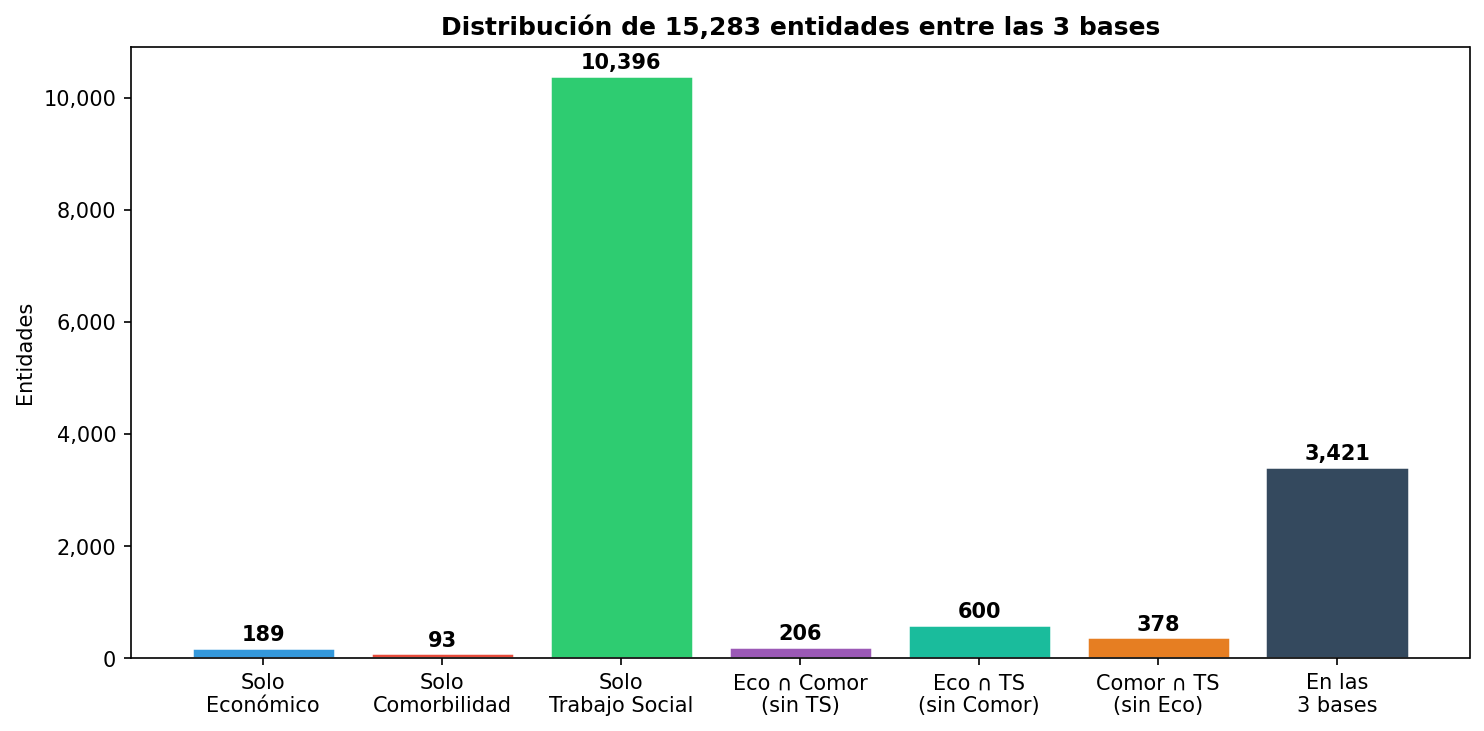
\includegraphics[width=\linewidth]{Figuras/distribucion_entidades.png}
\caption{Distribución de entidades únicas por región}
\label{fig:distribucion_entidades}
\end{figure}

\begin{figure}[H]
\centering
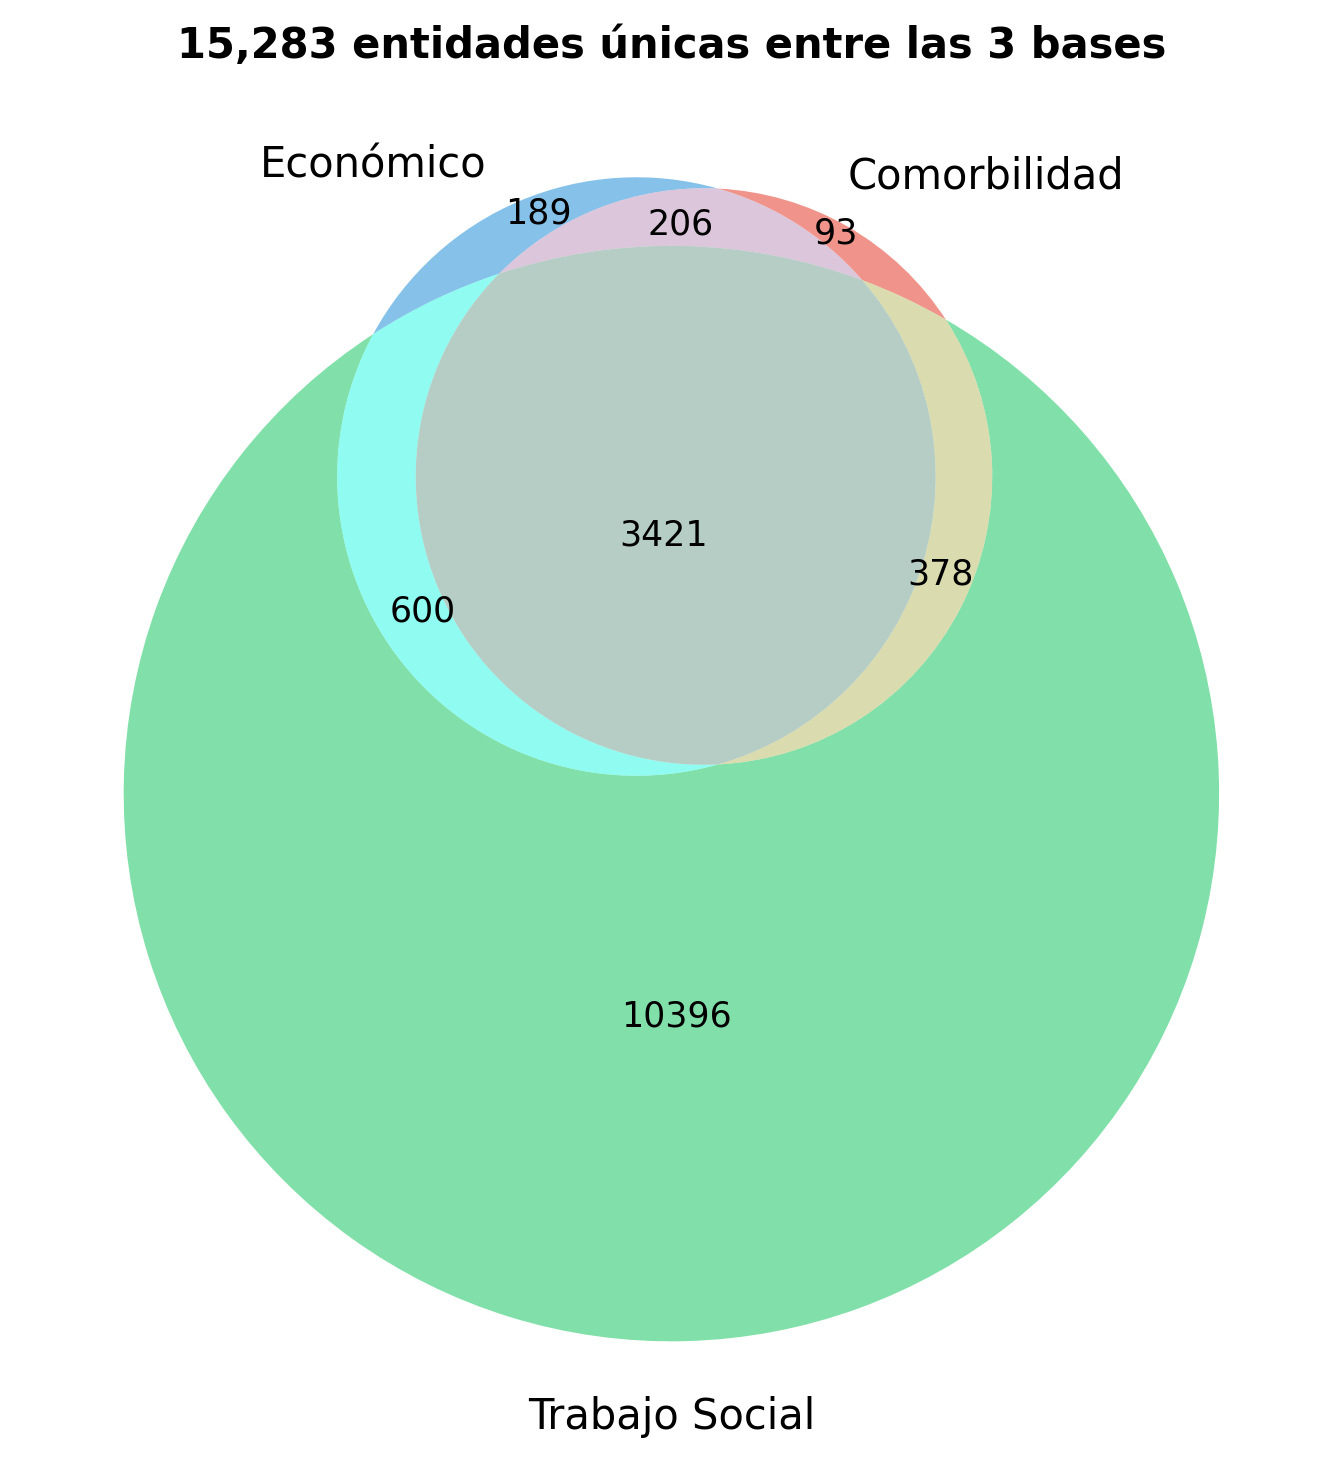
\includegraphics[width=0.75\linewidth]{Figuras/venn_entidades.png}
\caption{Diagrama de Venn: distribución de entidades entre las tres bases}
\label{fig:venn_entidades}
\end{figure}

La tabla~\ref{tab:sintesis_espacios} condensa el resultado completo de la vinculación oficial en dos paneles: las métricas a nivel de pares y las métricas a nivel de entidades.

\begin{table}[H]
\centering
\small
\caption{Síntesis del espacio de búsqueda y entidades vinculables}
\label{tab:sintesis_espacios}
\textbf{Pares de comparación}\\[2pt]
\begin{tabular}{lr}
\toprule
\textbf{Métrica} & \textbf{Valor} \\
\midrule
Espacio total cross-CSV               & 151,648,056 \\
Candidatos (vinculación oficial)      &      11,487 \\
\quad Llave exacta                    &       9,855 \\
\quad Métrica clásica                 &       1,118 \\
\quad Revisión manual                 &         514 \\
Positivos confirmados                 &      11,466 \\
Negativos confirmados                 &          21 \\
\bottomrule
\end{tabular}

\vspace{12pt}

\textbf{Entidades únicas}\\[2pt]
\begin{tabular}{lr}
\toprule
\textbf{Métrica} & \textbf{Valor} \\
\midrule
Registros totales (3 bases)            & 23,706 \\
Entidades únicas                        & 15,283 \\
Solo en una base                        & 10,678 \\
Vinculables (en $\geq$2 bases)          &  4,605 \\
$\bullet$ En exactamente 2 bases        &  1,184 \\
$\bullet$ En las 3 bases                &  3,421 \\
\bottomrule
\end{tabular}
\end{table}

Es importante señalar que este conjunto etiquetado constituye un \textit{silver standard}, no una verdad absoluta. Su construcción depende del número de expediente como filtro primario, lo que implica que cualquier paciente cuyo expediente difiera entre fuentes queda excluido de los candidatos, incluso si su nombre es semánticamente similar. Esta limitación es inherente al enfoque determinístico y motiva la transición hacia un modelo basado en representaciones semánticas, descrito en el Capítulo~4.

\section{Limitaciones}
\label{sec:limitaciones}

El pipeline descrito en las secciones anteriores operó bajo un esquema determinístico basado en reglas explícitas: filtrado por expediente, normalización de nombres, métricas de similitud clásica y revisión manual. Este enfoque fue suficiente para generar el \textit{silver standard}, pero dejó al descubierto tres limitaciones estructurales que motivan un cambio de paradigma.

La primera y más crítica es la \textbf{dependencia del número de expediente como filtro de candidatos}. Cualquier paciente cuyo expediente difiera entre fuentes queda automáticamente excluido del espacio de búsqueda, incluso si su nombre es semánticamente similar. El caso de los 80 registros con \texttt{EXP} nulo en Económico tratados como excepción mediante cruce por nombre evidencia esta fragilidad: un volumen mayor de expedientes faltantes habría requerido un enfoque diferente. La cobertura real del ground truth podría ser ligeramente superior a las 4,605 entidades vinculadas reportadas, pero el método determinístico no puede recuperar esos casos sin ampliar el filtro.

La segunda limitación es la \textbf{colisión de identificadores y el riesgo de falsos positivos por normalización}. En Económico se detectaron 6 expedientes asignados a nombres completamente distintos, lo que significa que un join por expediente sin validación cruzada genera pares espurios. Por otra parte, el ordenamiento alfabético de tokens ---necesario para resolver la diferencia de formato entre Comorbilidad y Económico--- introduce un riesgo: dos personas con los mismos apellidos y nombres, pero en orden diferente, colapsarían a la misma secuencia normalizada. En una base hospitalaria con apellidos frecuentes como García, López o Martínez este riesgo no es despreciable; aunque el expediente actúa como primer filtro, y la revisión manual confirmó 21 negativos explícitos, la prevención de este tipo de errores no puede garantizarse con reglas rígidas.

La tercera limitación es la \textbf{heterogeneidad estructural que impide la comparación directa del registro completo columna a columna}. Una misma variable ---el diagnóstico del paciente--- se representa como texto libre con codificación CIE-10 en Comorbilidad, como categórica de baja cardinalidad en Económico y como texto libre sin codificación en Trabajo Social. Las variables socioeconómicas como escolaridad u ocupación difieren incluso en el vocabulario: Económico emplea catálogos controlados mientras que Trabajo Social las captura como texto libre. Un esquema relacional tradicional requeriría armonizar todas estas representaciones antes de cualquier consulta, lo que resulta inviable cuando los sistemas de origen evolucionan de forma independiente, pero más interesante aún, cuando la información de un mismo paciente queda fragmentada en múltiples fuentes que no comparten el mismo esquema, algoritmos de comparación sintáctica como Jaro-Winkler o Levenshtein no pueden aplicarse de forma directa pues sus puntajes rara vez coinciden de forma consistente y requieren reglas condicionales que crecen en complejidad con cada nueva fuente haciendo que el proceso de ligado sea cada vez más frágil y costoso, llevando un mayor número de casos a revisión manual que podrían resolverse de forma automática si se contara con un modelo de \textbf{comparación semántica}.

Estas limitaciones comparten una causa común: el enfoque opera sobre la \textbf{representación tabular} de los datos, donde cada columna tiene un formato, un orden y un vocabulario definidos por el sistema de origen. La información del mismo paciente queda fragmentada en esquemas inconexos que solo pueden reconciliarse mediante  intervención humana para resolver casos ambiguos.

La alternativa que se explora en el Capítulo~4 consiste en trascender la representación tabular y comparación sintáctica y operar sobre una \textbf{abstracción semántica} del paciente: representar cada registro como un conjunto de \textbf{bloques de información comparables} (diagnóstico clínico, perfil demográfico, situación socioeconómica) independientemente de cómo estén codificados en la base original, y comparar los registros completos mediante representaciones vectoriales aprendidas. Este cambio de paradigma, de la comparación de caracteres en cada columna a la comparación semántica de entidades, es el núcleo metodológico de la propuesta en el siguiente capítulo.